\section{Metodologia}
\begin{frame}{Metodologia}
	\begin{enumerate}
	    \item Desenvolver uma ferramenta em linha de comando para ser usado em \textit{user-space}
	    \item Migrar o código para o U-Boot
	    \begin{itemize}
	        \item Implementar a API de sistemas de arquivo do U-Boot
	        \item Implementar os comandos do U-Boot
	    \end{itemize}
	    \item Submeter o trabalho na \textit{mailing list} do U-Boot
	\end{enumerate}
\end{frame} 

\begin{frame}{Ferramenta de linha de comando: \textit{squashfs-utils}}
	\begin{itemize}
	    \item Ferramenta: \textit{squashfs-utils}
	    \item Construída \textit{from scratch}, usando uma documentação não-oficial do SquashFS
	    \item Entender como o sistema de arquivos se organiza
	    \item Definir estruturas de dados essenciais
	    \item Analisar e imprimir as seções da imagem SquashFS
	\end{itemize}
\end{frame}

\begin{frame}{Gerando uma imagem SquashFS}
    \begin{figure}
        \centering
        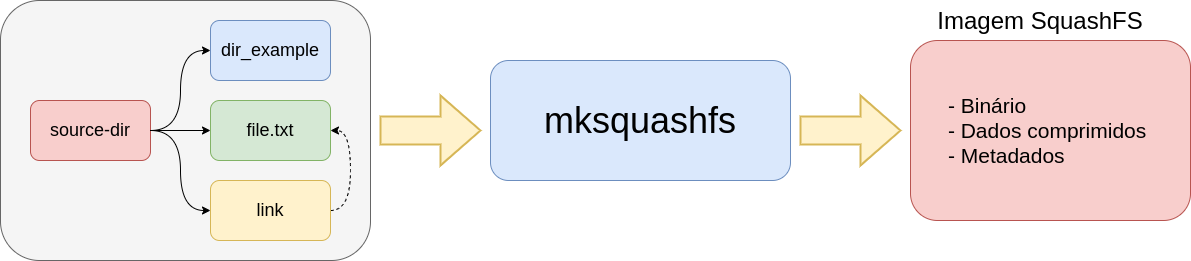
\includegraphics[scale=0.25]{figuras/mksquashfs.png}
        \caption{Compilação de uma imagem SquashFS}
        \label{fig:my_label}
    \end{figure}
\end{frame}

\begin{frame}{Imagem SquashFS}
    \begin{figure}
        \centering
        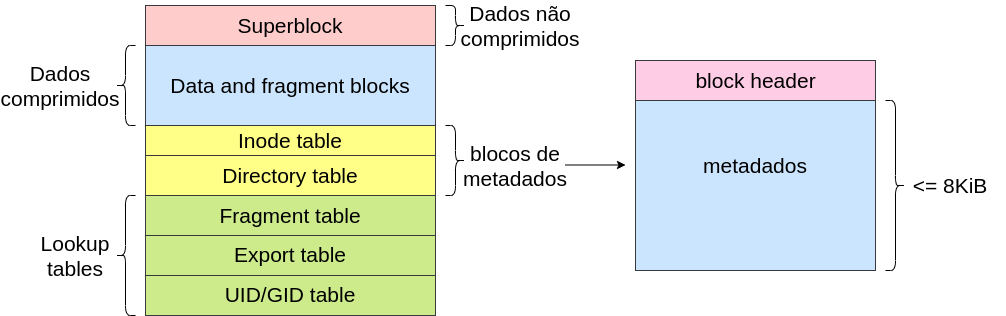
\includegraphics[scale=0.32]{figuras/sqfs.png}
        \caption{Layout de uma imagem SquashFS}
        \label{fig:my_label}
    \end{figure}
\end{frame}

\begin{frame}{Ferramenta de linha de comando: \textit{squashfs-utils}}
    \begin{figure}
        \centering
        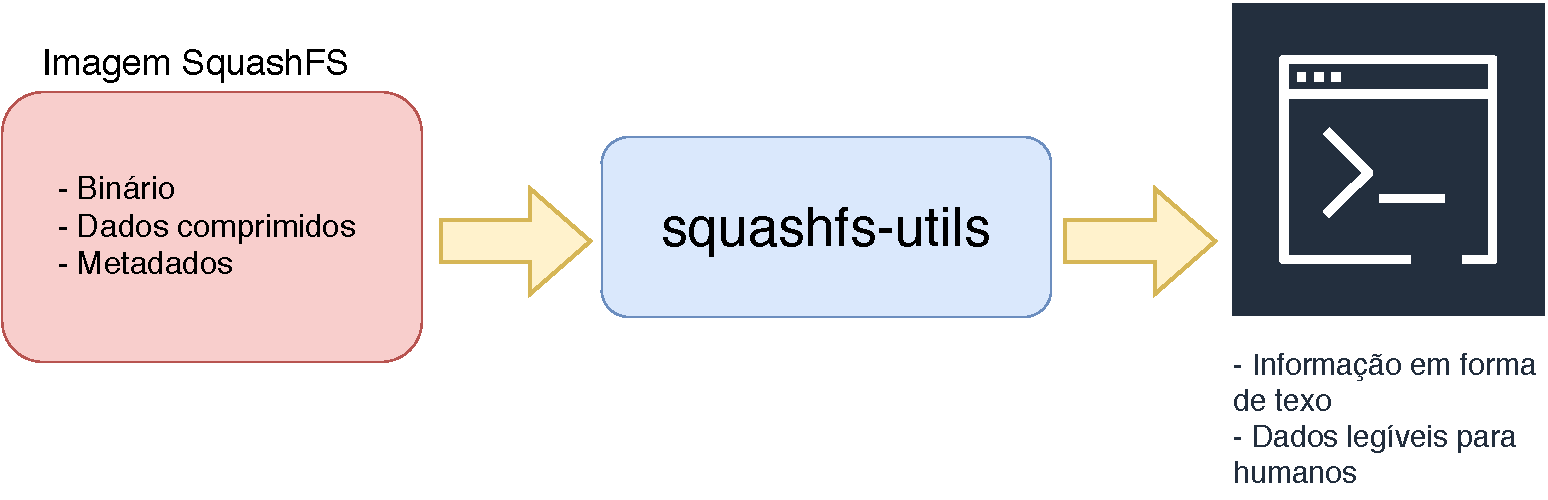
\includegraphics[scale=0.4]{figuras/sqfsutils.pdf}
        \caption{Uso da \textit{squashfs-utils}}
        \label{fig:my_label}
    \end{figure}
\end{frame}

\begin{frame}{Ferramenta de linha de comando: \textit{squashfs-utils}}
Vamos executar alguns comandos para analisar uma imagem SquashFS gerada a partir do diretório abaixo:
\begin{figure}
    \centering
    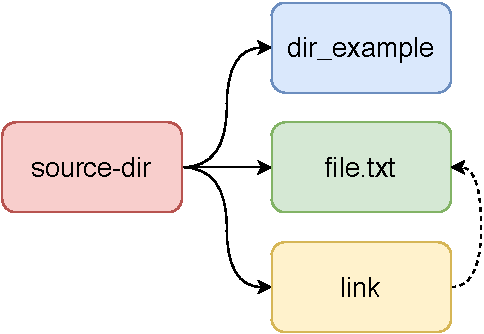
\includegraphics[scale=0.7]{figuras/tree.pdf}
    \caption{Diretório fonte: diretório vazio, arquivo de texto e link simbólico}
    \label{fig:my_label}
\end{figure}
\end{frame}


\begin{frame}[fragile]{Ferramenta de linha de comando: \textit{squashfs-utils}}

Instruções de uso:

\begin{minted}[fontsize=\fontsize{8}{8}, bgcolor=blcodebg]{text}
$ ./sqfs -h
usage: sqfs [-h]
       sqfs [-s] [-i] [-d] <fs-image>
       sqfs [-e] <fs-image> /path/to/dir/
       sqfs [-e] <fs-image> /path/to/file

Tool to analyze the content of a SquashFS image

Options:
       -h: Prints the usage and exits
       -s: Dumps the contents of a SquashFS image's superblock
       -i: Dumps the contents of a SquashFS image's inode table
       -d: Dumps the contents of a SquashFS image's directory table
       -e: Dumps the contents of a SquashFS image's file or directory.
       For directories, end path with '/'.

Parameters:
       <fs-image>: Path to the filesystem image
\end{minted}    
\end{frame}


\begin{frame}[fragile]{Ferramenta de linha de comando: \textit{squashfs-utils}}
Informações do \textit{Superblock}:
\begin{minted}[fontsize=\fontsize{7}{7}, bgcolor=blcodebg]{text}
$./sqfs -s source-dir.sqfs 
--- SUPER BLOCK INFORMATION ---
Magic number: sqsh
Number of inodes: 4
Filesystem creation date: Tue 2020-08-04
(yyyy-mm-dd) 15:46:14 CEST
Block size: 131 kB
Number of fragments: 1
Block log: 17
Compression type: ZLIB
Super Block Flags: 0xc0
Major/Minor numbers: 4/0
Root inode: 0x60
Bytes used: 312
Id table start: 0x130
(xattr) Id table start: 0xffffffffffffffff
Inode table start: 0x6c
Directory table start: 0xbc
Fragment table start: 0x105
Lookup table start: 0x122
--- SUPER BLOCK FLAGS ---
Duplicates
Exportable

\end{minted}    
\end{frame}

\begin{frame}[fragile]{Ferramenta de linha de comando: \textit{squashfs-utils}}
Informações da \textit{Inode table}:
   \begin{columns}
   \begin{column}{0.5\textwidth}

\begin{minted}[fontsize=\fontsize{5}{5}, bgcolor=blcodebg]{text}
$./sqfs -i source-dir.sqfs
--- --- ---
{Inode 1/4}
--- --- ---
Permissions: 0x01fd
UID index: 0x0000
GID index: 0x0000
Modified time: Tue 2020-08-04 (yyyy-mm-dd) 15:41:41 CEST
Inode number: 1
Inode type: Basic Directory
Start block: 0x00000000
Hard links: 2
File size: 3
Block offset: 0x0000
Parent inode number: 4

{Inode 2/4}
--- --- ---
Permissions: 0x01b4
UID index: 0x0000
GID index: 0x0000
Modified time: Tue 2020-08-04 (yyyy-mm-dd) 15:42:17 CEST
Inode number: 2
Inode type: Basic File
Start block: 0x00000000
Fragment block index: 0x00000000
Fragment block offset: 0x00000000
(Uncompressed) File size: 12
\end{minted}
   \end{column}
   \begin{column}{0.5\textwidth}
\begin{minted}[fontsize=\fontsize{5}{5}, bgcolor=blcodebg]{text}
{Inode 3/4}
--- --- ---
Permissions: 0x01ff
UID index: 0x0000
GID index: 0x0000
Modified time: Tue 2020-08-04 (yyyy-mm-dd) 15:45:48 CEST
Inode number: 3
Inode type: Basic Symlink
Hard links: 1
Symlink size: 8
Target path: file.txt

{Inode 4/4}
--- --- ---
Permissions: 0x01fd
UID index: 0x0000
GID index: 0x0000
Modified time: Tue 2020-08-04 (yyyy-mm-dd) 15:45:48 CEST
Inode number: 4
Inode type: Basic Directory
Start block: 0x00000000
Hard links: 3
File size: 63
Block offset: 0x0000
Parent inode number: 5
\end{minted}
   \end{column}
   \end{columns}
\end{frame}

\begin{frame}[fragile]{Ferramenta de linha de comando: \textit{squashfs-utils}}
Informações da \textit{Directory table}:

\begin{minted}[fontsize=\fontsize{9}{9}, bgcolor=blcodebg]{text}
$./sqfs -d source-dir.sqfs
Directory 1
Name: dir_example
Empty directory.

Root directory
1) dir_example
2) file.txt
3) link
\end{minted}
\end{frame}

\begin{frame}[fragile]{Ferramenta de linha de comando: \textit{squashfs-utils}}
Recuperando o conteúdo de um arquivo:
\begin{minted}[fontsize=\fontsize{9}{9}, bgcolor=blcodebg]{text}
$ cat source-dir/file.txt
Hello world

$./sqfs -e source-dir.sqfs /file.txt
Hello world
\end{minted}
\end{frame}

\begin{frame}{Migração do código para o U-Boot}
    \begin{figure}
        \centering
        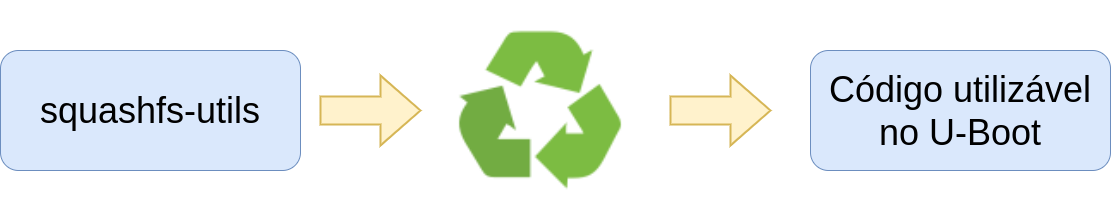
\includegraphics[scale=0.27]{figuras/recycle_transparente.png}
        \caption{Adaptação do código da \textit{squashfs-utils}}
        \label{fig:my_label}
    \end{figure}
\end{frame}

\begin{frame}{Migração do código para o U-Boot}
    \begin{figure}
        \centering
        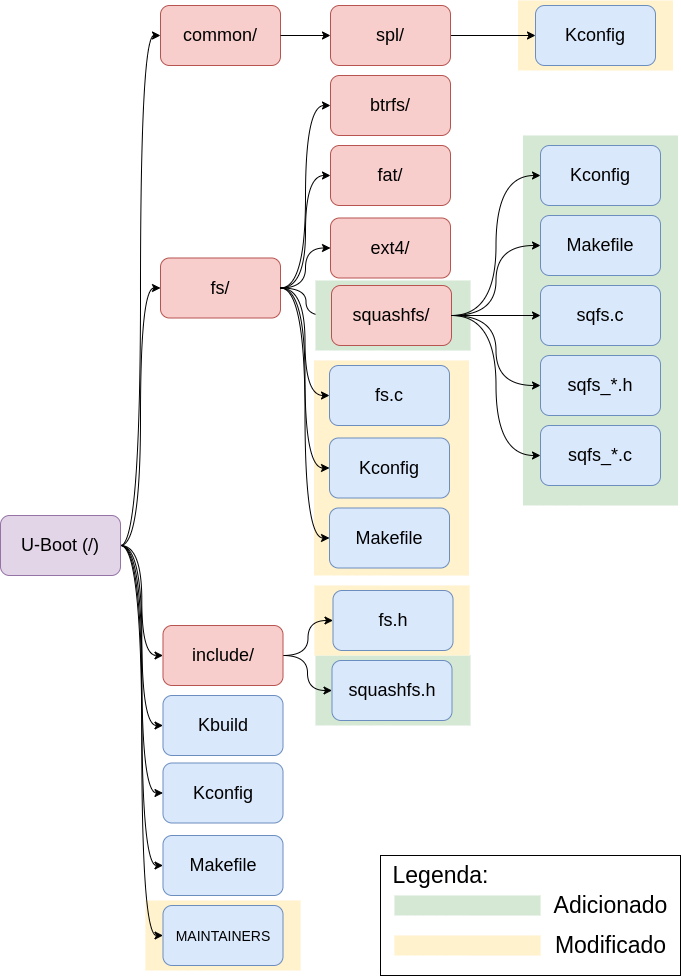
\includegraphics[scale=0.185]{figuras/uboot.png}
        \caption{Diretório raiz do U-Boot}
        \label{fig:my_label}
    \end{figure}
\end{frame}

\begin{frame}{Implementação da API para sistemas de arquivo do U-Boot}
\begin{figure}
    \centering
    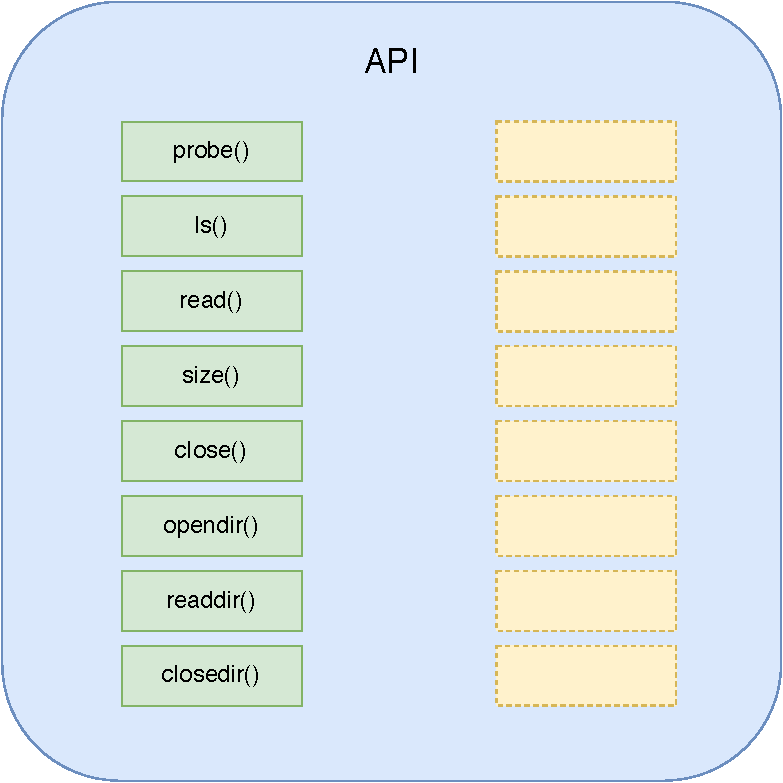
\includegraphics[scale=0.45]{figuras/API.pdf}
    \caption{Funções da API para sistemas de arquivo}
    \label{fig:my_label}
\end{figure}
\end{frame}

\begin{frame}{Implementação da API para sistemas de arquivo do U-Boot}
\begin{figure}
    \centering
    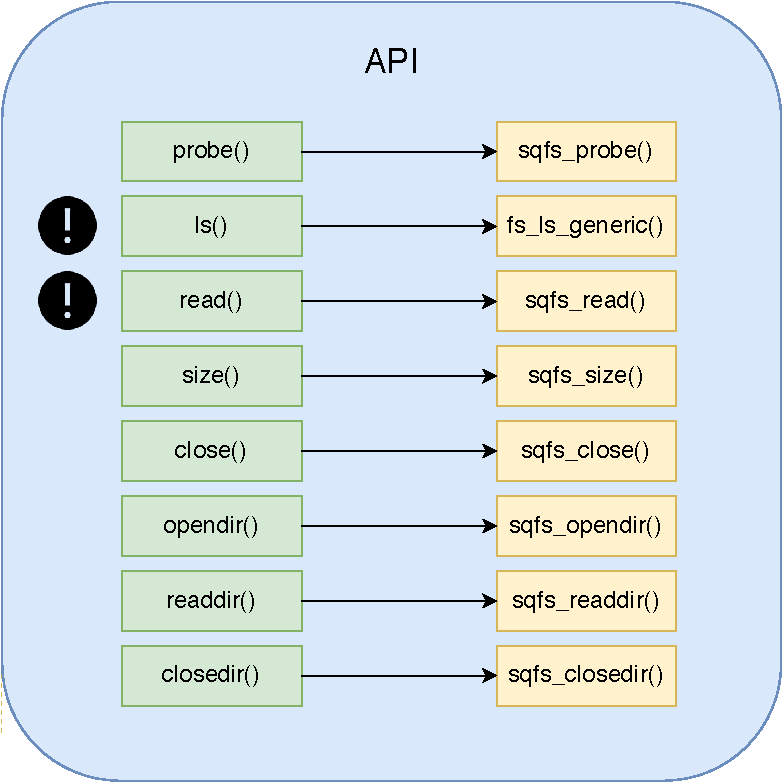
\includegraphics[scale=0.45]{figuras/API2.pdf}
    \caption{Implementação da API para o SquashFS}
    \label{fig:my_label}
\end{figure}
\end{frame}


\begin{frame}[fragile]{Implementando os comandos do U-Boot}

Comando \textit{ls} (\textit{sqfsls}):

\begin{minted}[fontsize=\fontsize{5}{5}, bgcolor=blcodebg]{text}
=> sqfsls 
sqfsls - List files in directory. Default: root (/).

Usage:
sqfsls <interface> [<dev[:part]>] [directory]
    - list files from 'dev' on 'interface' in 'directory'

\end{minted}
\end{frame}

\begin{frame}[fragile]{Implementando os comandos do U-Boot}

Comando \textit{load} (\textit{sqfsload}):

\begin{minted}[fontsize=\fontsize{5}{5}, bgcolor=blcodebg]{text}
=> sqfsload 
sqfsload - load binary file from a SquashFS filesystem

Usage:
sqfsload <interface> [<dev[:part]> [<addr> [<filename> [bytes [pos]]]]]
    - Load binary file 'filename' from 'dev' on 'interface'
      to address 'addr' from SquashFS filesystem.
      'pos' gives the file position to start loading from.
      If 'pos' is omitted, 0 is used. 'pos' requires 'bytes'.
      'bytes' gives the size to load. If 'bytes' is 0 or omitted,
      the load stops on end of file.
      If either 'pos' or 'bytes' are not aligned to
      ARCH_DMA_MINALIGN then a misaligned buffer warning will
      be printed and performance will suffer for the load.
\end{minted}

\end{frame}

\begin{frame}{Implementando os comandos do U-Boot}
\begin{figure}
    \centering
    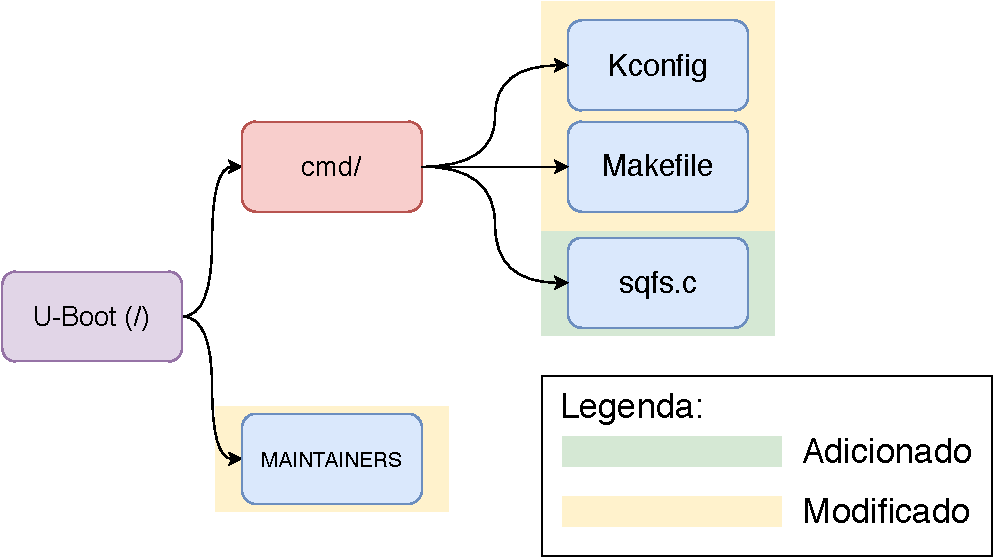
\includegraphics[scale=0.55]{figuras/uboot-commands.pdf}
    \caption{Diretório raiz do U-Boot}
    \label{fig:my_label}
\end{figure}
\end{frame}

\begin{frame}{Scripts de teste}
    Scripts escritos em Python para testar os comandos do SquashFS: \textit{sqfsload} e \textit{sqfsls}
    
    \begin{figure}
        \centering
        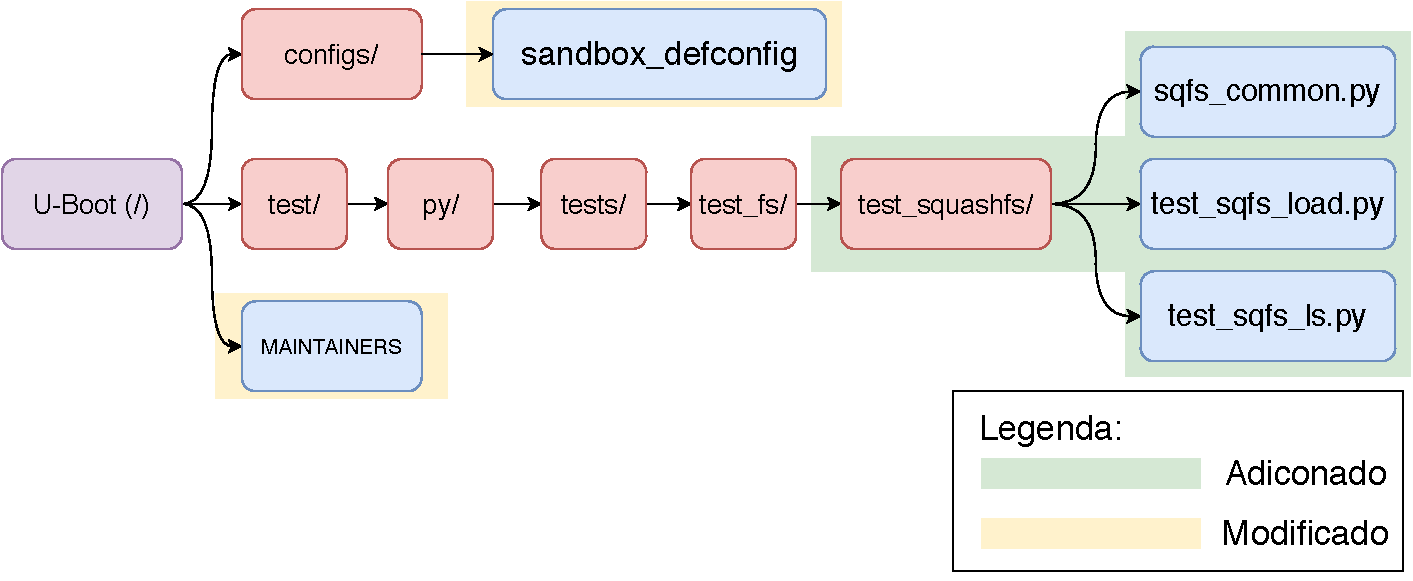
\includegraphics[scale=0.4]{figuras/tests.pdf}
        \caption{Diretório raiz do U-Boot}
        \label{fig:my_label}
    \end{figure}
\end{frame}

\begin{frame}{Submissão do trabalho na mailing list do U-Boot}
   \begin{columns}
   \begin{column}{0.5\textwidth}
\begin{itemize}
\item Consertar todos os problemas de estilo
\item Escrever uma carta de apresentação
\item Dividir o trabalho em \textit{patches}
\end{itemize}
   \end{column}

   \begin{column}{0.5\textwidth}
   Patches:
   \begin{enumerate}
   \item fs/squashfs: new filesystem
   \item cmd/: add filesystem commands
   \item include/u-boot, lib/zlib: add sources for zlib decompression
   \item fs/squashfs: add support for zlib decompression
   \item fs/fs.c: add symbolic link case to fs\_ls\_generic()
   \item test/py: Add tests for the SquashFS commands
   \end{enumerate}
   \end{column}
   \end{columns}
\end{frame}

\begin{frame}{Metodologia de trabalho}
\begin{figure}
    \centering
    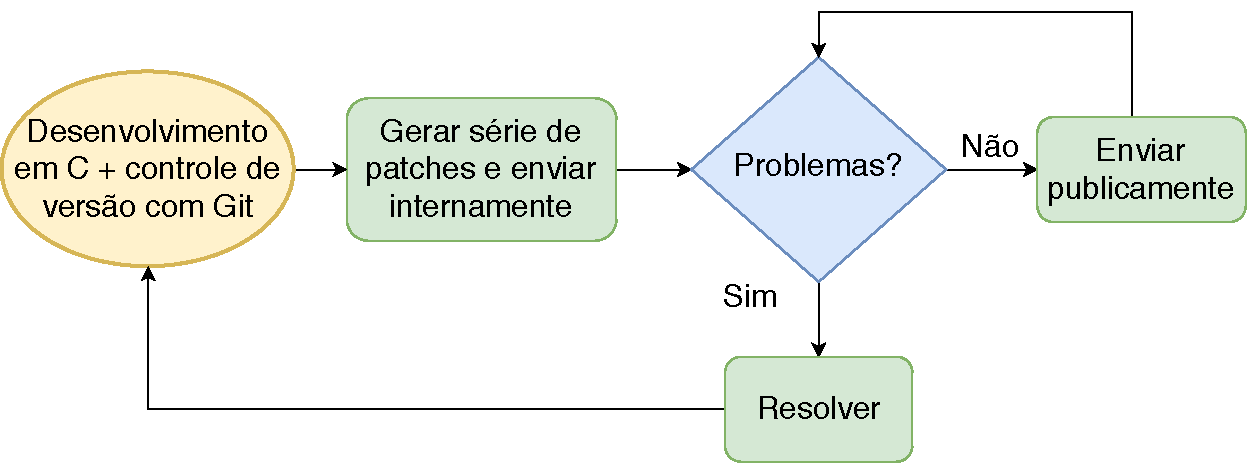
\includegraphics[scale=0.5]{figuras/workflow.pdf}
    \caption{Fluxograma da metodologia}
    \label{fig:my_label}
\end{figure}
\end{frame}

\begin{frame}{Metodologia de trabalho}

Execuções do código feitas na \textit{Sandbox} do U-Boot e numa Beagle Bone Black Wireless:

\begin{figure}
    \centering
    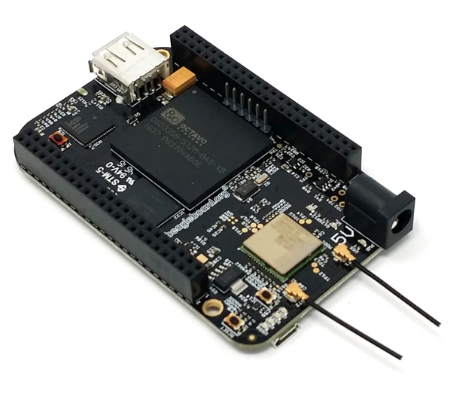
\includegraphics[scale=0.3]{figuras/bbb.png}
    \caption{Beagle Bone Black Wireless}
    \label{fig:my_label}
\end{figure}
\end{frame}

\begin{frame}[fragile]{Resultados}
Console do U-Boot, lançado na Beagle Bone Black Wireless:
\begin{minted}[fontsize=\fontsize{4}{4}, bgcolor=blcodebg]{text}
U-Boot SPL 2020.10-rc1-00154-gc7b2d6a45d (Aug 07 2020 - 11:17:02 +0200)
Trying to boot from MMC1

U-Boot 2020.10-rc1-00154-gc7b2d6a45d (Aug 07 2020 - 11:17:02 +0200)

CPU  : AM335X-GP rev 2.1
Model: TI AM335x BeagleBone Black
DRAM:  512 MiB
WDT:   Started with servicing (60s timeout)
NAND:  0 MiB
MMC:   OMAP SD/MMC: 0, OMAP SD/MMC: 1
Loading Environment from FAT... Unable to use mmc 0:1... <ethaddr> not set.
Validating first E-fuse MAC
Net:   Could not get PHY for ethernet@4a100000: addr 0
eth2: ethernet@4a100000, eth3: usb_ether
Hit any key to stop autoboot:  0
=> sqfsls mmc 0:1
            bin/
            boot/
            dev/
            etc/
            lib/
    <SYM>   lib32
    <SYM>   linuxrc
            media/
            mnt/
            opt/
            proc/
            root/
            run/
            sbin/
            sys/
            tmp/
            usr/
            var/

2 file(s), 16 dir(s)
\end{minted}
\end{frame}

\begin{frame}[fragile]{Resultados}
Carregando o kernel e a device tree:
\begin{minted}[fontsize=\fontsize{7}{7}, bgcolor=blcodebg]{text}
=> sqfsload mmc 0:1 $kernel_addr_r /boot/zImage
6091376 bytes read in 476 ms (12.2 MiB/s)
=> sqfsload mmc 0:1 $fdt_addr_r /boot/am335x-boneblack.dtb
40817 bytes read in 14 ms (2.8 MiB/s)
=> setenv bootargs console=ttyO0,115200n8
=> bootz $kernel_addr_r - $fdt_addr_r
## Flattened Device Tree blob at 81000000
   Booting using the fdt blob at 0x81000000
   Loading Device Tree to 8fff3000, end 8fffff70 ... OK

Starting kernel ...

[    0.000000] Booting Linux on physical CPU 0x0
[    0.000000] Linux version 4.19.79 (joaomcosta@joaomcosta-Latitude-E7470)
(gcc version 7.3.1 20180425 [linaro-7.3-2018.05 revision
d29120a424ecfbc167ef90065c0eeb7f91977701] (Linaro GCC 7.3-2018.05))
#1 SMP Fri May 29 18:26:39 CEST 2020
[    0.000000] CPU: ARMv7 Processor [413fc082] revision 2 (ARMv7), cr=10c5387d
\end{minted}
\end{frame}


\begin{frame}{Resultados}
\begin{itemize}
\item O suporte do SquashFS foi aceito e integrado ao código oficial do U-Boot
\begin{figure}
\centering
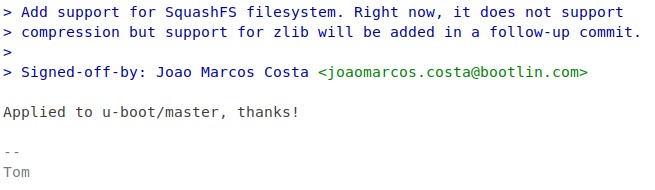
\includegraphics[scale=0.4]{figuras/tom.jpeg}
\caption{Mensagem de aceite de Tom Rini, administrador principal do U-Boot}
\end{figure}
\item Balanço final: 27 arquivos novos e/ou modificados e aproximadamente 3000 linhas de código
\end{itemize}
\end{frame}


